\documentclass[10pt,twocolumn]{article}
\usepackage[english]{babel}
\usepackage{amssymb}
\usepackage{amsmath}
\usepackage[left=1.5cm, right=1.5cm]{geometry}
\usepackage{csquotes}
\usepackage{caption}
\usepackage{graphicx}
\usepackage{multicol}
\usepackage[dvipsnames]{xcolor}
\usepackage[backend=biber,sorting=none]{biblatex}
\addbibresource{references.bib}
% \graphicspath{ {./images/} }


\begin{document}

\title{Computational Neuroscience: \\ Inhibitory-Stabilised Networks}
\author{B204511}
\date{November 2024}
\maketitle

\section{Introduction}
Several brain regions, including the neocortex and hippocampus \cite{tsodyks1997paradoxical}
contain local recurrently connected networks of excitatory and inhibitory neurons.
Understanding how those networks function and react to external inputs is important
for analysing how the brain operates. This report will introduce the concept of
such networks, discuss their biological relevance, present a mathematical model, and provide
computer simulations as well as mathematical analysis of the model.

The network is viewed as consisting of 2 pools of neurons: excitatory and inhibitory.
Each pool projects to the other, and to itself, forming a recurrent neural network.
Excitatory feedback can lead to runaway excitation, which is prevented by the inhibitory feedback.
This allows the network to stabilise, earning it the name Inhibitory-Stabilised Network (ISN).


To understand how the system comes together, it is important to get a sense of what
the underlying model of each individual nueron is and how the interaction between them integrates.

% #######################
% Model of the Neuron
% #######################

\subsection{Leaky Integrate-and-Fire Neuron}
In 1907, Louis Édouard Lapicque \cite{brunel2007quantitative} introduced
the concept of the integrate-and-fire neuron model.
Even though the model was developed before scientists
had a chance to describe the biophysical mechanics of the neuron,
it captured the behaviour of the neuron in a way that was useful
for understanding \cite{abbott1999lapicque}.

The neuron is viewed as an electric circuit with a capacitor and a resistor connected in parallel.
% resistor
The membrane has some resistance, which is assumed to be constant and can be described by Ohm's law: $V = IR$, and therefore
the resistor current is $I = \frac{V}{R} = gV$, where $g$ is conductance of the cell.
% capacitor
The relationship between the current and the voltage across the capacitor is described by the following equation:
$C = \frac{Q}{V}$, where $C$ is the capacitance, $Q$ is the charge stored in the capacitor, and $V$ is the voltage across the capacitor.
Knowing this, the current in the circuit:

$$
    I = \frac{dQ}{dt} = \frac{dCV}{dt} = C \frac{dV}{dt}
$$
% Combining the two, we get: $C \frac{dV}{dt} = gV$.

Real neurons, however, receive current from other neurons via dendrites from synapses,
and induce own \textbf{ionic} current by
% opening and closing ion channels (each with its own conductance) and 
letting charged particles
% ($Na^+, Cl^-, Ca^{2+}, K^+$) 
in and out of the cell. Therefore,
the total current is the sum of the ionic current plus any external input: $I = \sum_{i}g_iV + I_{ext} = g_mV + I_{ext}$.
Neurons are generally \textbf{negatively charged} relative to the outside, and therefore the flow outside the cell is treated as positive.
Since the size of the cell and its channels is comparable to that of ions, effect of electric attraction is comparable with that of diffusion,
and there exists a point, where one balances out the other, resulting in the zero net current flow.
This point is called the resting potential $V_{rest}$ of the neuron, and therefore any current should be measured relative to this potential.

$$
    C \frac{dV}{dt} = -g_m(V - V_{\text{rest}}) + I_{\text{ext}}
$$

Dividing by conductance, we get the following equation:
$$
    \tau_m \frac{dV}{dt} = -(V - V_{\text{rest}}) + \frac{I_{\text{ext}}}{g_m}
$$
where $\tau_m$ is the membrane time constant, describing how quickly it reacts to input.

Now, the external current is the component of interest,
by extending this component, we can integrate input from other neurons.
Neurons communicate by sending electrical signals to each other, via the synapse of
emitting through the dendrites of the receiving neuron.
This interaction can be modelled as a synpatic current, weighted by the strength of connection.
Dale's Law\cite{efron1968psychopharmacology} states that a neuron can only be
either excitatory or inhibitory, and therefore we can simplify the model, and
approximate the synaptic current as a function of emitting neuron's voltage:
$I_{\text{syn},i} = W\phi(V_i)$,
where $W$ is the synaptic weight ($+$ for excitatory, $-$ for inhibitory), and $\phi(V)$ is the transfer function of the neuron.
The actual external current collapses into $I_{ext}/g_m=u_{ext}$.

Combing all component, we obtain a system of equations:
\begin{equation}
    \tau_E \frac{dV_E}{dt} =
    -(V_E - V_{\text{rest}})
    + W_{EE} \phi(V_E)
    - W_{EI} \phi(V_I) + u_E
\end{equation}

\begin{equation}
    \tau_I \frac{dV_I}{dt} =
    -(V_I - V_{\text{rest}})
    + W_{IE} \phi(V_E)
    - W_{II} \phi(V_I) + u_I
\end{equation}
where $V_{\text{rest}}$ is the resting potential of the neuron, $W_{k}$ are the
synaptic weights, $u_k$ are the external inputs to neurons,
and $\phi(V)$ is the transfer function of a neuron, that acts as
a communication channel between the neurons and is defined as a scaled ReLU function:

\begin{equation}
    \phi(V) = \beta[V-V_0]_+
\end{equation}

Now that we have the model and its origins, it's important to outline
the benefits and limitations of the model.

\subsection{Considerations (Q1)}
1. The model abstracts away certain biological complexity, such as stochasticity and
variability of individual ion channels (both in somas and synapses), described in
great detail by the Hodgkin-Huxley model \cite{hodgkin1952quantitative}, which is
a more biologically plausible model of the neuron,
but is also signficantly more complex.

2. Synaptic weights are a heuristic approximation of synpatic conductances
and assumed to be constant, whereas in reality they are
subject to plasticity, and can change over time.

3. The input activity from the opposite neural pool is treated as a
linear function of its voltage with an activation threshold,
which is not realistic as neurons spiking activity varies depending
on its structure and intrinsic properties \cite{izhikevich2003simple}.

3. The membrane time constant that comes from conductance is assumed
to be constant, and its usage relies on Ohm's law holding, which is
a simplification of the actual behaviour of a neuron.
However, it is a good approximation for the passive dynamics of a neuron
which makes the model tractable for analysis.

4. The LIF model is a lot more computationally affordable, requires 4 ODEs
per neuron in the HH model, instead of 1 in the LIF model,
which allows us to run large scale simulations and analyse
the network behaviour faster. The model is also more amenable
to theoretic analysis, which helps to explain certain activity patterns in the network.

In essence, we trade off biological accuracy for
computational efficiency and analytic tractability.


% ####################### 
% COMPUTER SIMULATIONS
% #######################

\section{Computer Simulations}
In this section, simulations of the network are presented,
where the network is stimulated with various external inputs for
both excitatory and inhibitory pools, and the
response of the network is approximated numerically using the Euler method.
Python code used for simulations can be found in Appendix A.

In our simulations, we study 2 networks with the following base parameters:
% V_rest
$$
    V_{\text{rest}} = -70 \text{mV, } V_0 = -55 \text{mV, } \beta = 1
$$

% tau
$$
    \tau
    = \begin{pmatrix} \tau_E \\ \tau_I \end{pmatrix}
    = \begin{pmatrix} 20 \\ 10 \end{pmatrix}\text{ms}
$$

% Us
$$
    u
    = \begin{pmatrix} u_E \\ u_I \end{pmatrix}
    = \begin{pmatrix} 20 \\ 20 \end{pmatrix}
$$

% Ws
$$
    W
    = \begin{pmatrix} W_{EE} & W_{EI} \\ W_{IE} & W_{II} \end{pmatrix}
    = \begin{pmatrix} W^n_{EE} & 0.65 \\ 1.2 & 0.5 \end{pmatrix}
$$

where $W^n_{EE}$ is the weight of the excitatory feedback for a given network.
The 2 networks differ in the weight of the excitatory feedback, where one is weaker
is $W^1_{EE} = 0.5$ and the other is stronger $W^2_{EE} = 1.25$.

\begin{figure*}
    \centering
    \captionsetup{justification=centering}
    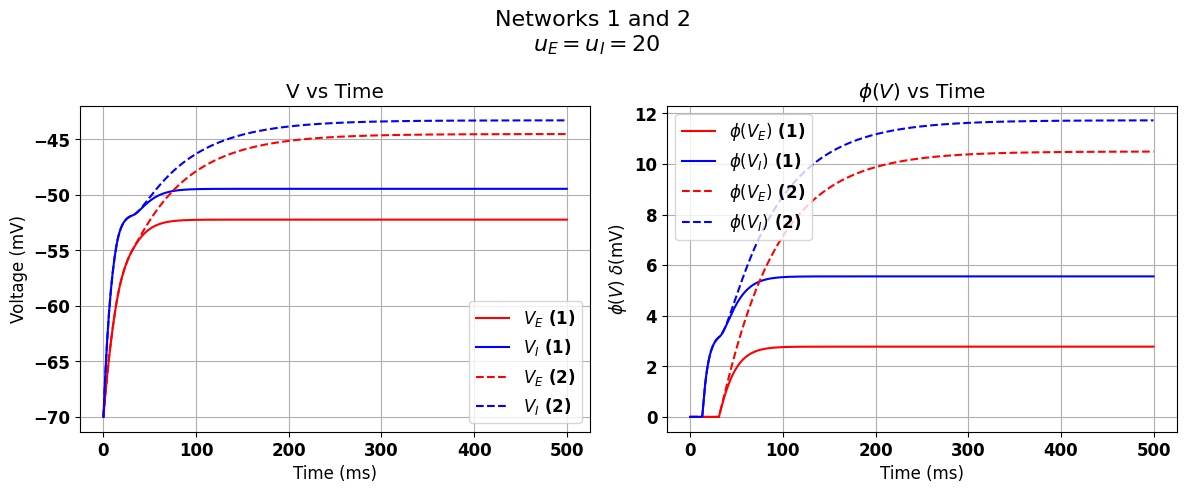
\includegraphics[width=1\textwidth]{images/12-stable.png}
    \caption{
        \textbf{Stable} external input to both neurons.\\
        \textcolor{red}{Excitatory} potentials are red, \textcolor{blue}{Inhibitory} potentials are blue. \\
        Network 1 is solid, Network 2 is dashed.
    }
    \label{fig:stable-input}
\end{figure*}

\subsection{Stable External Input (Q2)}
We first study both networks subjected to a stable external input of 20mV to
both neurons.
Both neurons start from the resting potential. The simulation is ran for 500ms
with 1ms time steps. The results are shown in Figure \ref{fig:stable-input}.

Looking at the results for Network 1 (solid lines), we can see that both neurons
gradually begin responding to the external input. Since $\tau_I < \tau_E$,
one might expect the \textcolor{blue}{inhibitory} neuron to respond faster, which is
exactly what is observed. The transfer function $\phi(V)$ is not immediately
responding to the increase in voltage as both neurons have to reach the threshold
potential, which matches with the timeline of both neurons reaching $V_0=-55mV$
and begin firing to provide input to the other. After about $5\tau$, as
expected with a capacitor behaviour, the system reaches a stable state
and both neurons' activity plateaus. At this point, $V_I$, however,
is about 3mV above $V_E$, which could be due to a stronger $W_{IE}$ connection
relative to $W_{EI}$, given that the feedback strength to both neurons is equal,
excitation of I is stronger than inhibition of E, and therefore less $V_E$
is needed to balance out $V_I$.

\subsection{Inhibitory Input Increase (Q3-4)}
\begin{figure*}
    \centering
    \captionsetup{justification=centering}
    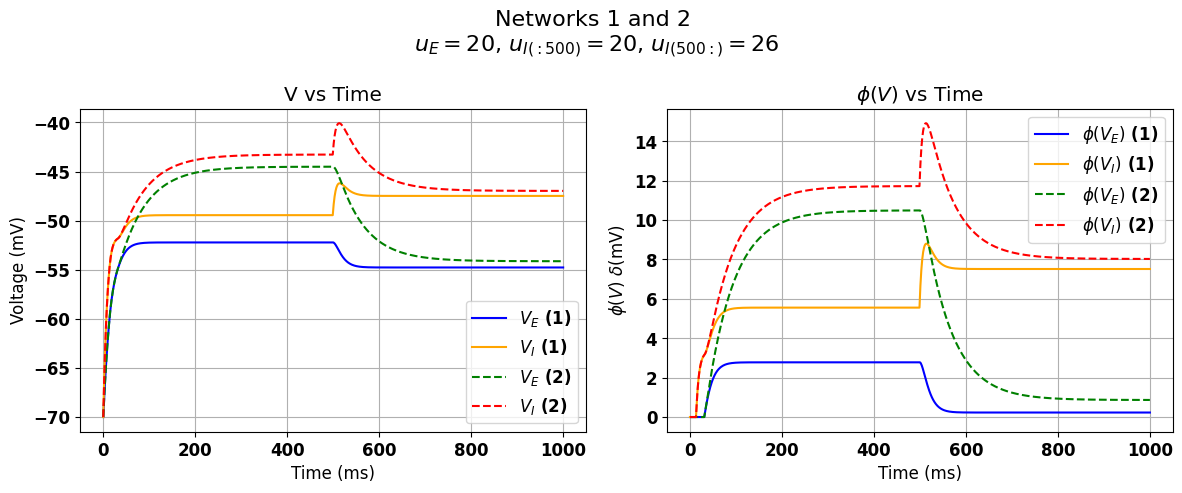
\includegraphics[width=1\textwidth]{images/12-I_input.png}
    \caption{External \textbf{inhibitory} input increase after 500ms.\\
        \textcolor{red}{Excitatory} potentials are red, \textcolor{blue}{Inhibitory} potentials are blue.\\
        Network 1 is solid, Network 2 is dashed.}
    \label{fig:i-input}
\end{figure*}

Both networks are simulated for further 500ms with
an increase in $u_I$ from $20$mV to $26$mV. The results for
this simulation are shown in Figure \ref{fig:i-input}.

Network 1, prior to the $u_I$ increase, is in a stable state, and immediately after
inhibitory activity naturally increases. As $V_I$ increases, according to
eqaution (1), $V_E$ decreases, which is expected. 10ms later, inhibitory activity
peaks and then drops slightly to stabilise once again, the peak and drop can be
explained by equation (2), that tells us that $V_I$ depends on weighted ReLU'd
activity of $V_E$, which has been decreasing previously and therefore at some point
decreasing excitatory activity will begin balancing out external inhibitory input
and we'd expect the network to begin approaching a stable state. Stable state
is eventually reached at about 570ms, where potentials settle once again, however,
$V_I$ is above its previous stable value, and $V_E$ is below. This makes sense
following the logic from the stable external input simulation - stronger $W_{IE}$
connection tells us that less excitatory activity is needed to
balance out the inhibitory.

For Network 2 (dashed lines), the results are similar but with a subtle difference. Both pools
are responding to the input as described above: inhibitory spike, then excitatory dip,
followed by the dip in inhibitory activity and eventual stabilisation. However,
this time round, the final stable state is below the original for both neurons,
which seems counterintuitive as the increase in inhibitory activity leads
to a reduction in the activity of the whole network. The paradox here would
be that, for some reason, the activity is not balancing like in Network 1,
but decreases overall. Since the only parameter that differs is the
$W_{EE}$ synaptic weight, the behaviour can attributed to it.

\subsection{Excitatory Input Increase (Q5)}
We will now simulate an increase in external Excitatory input, unlike Inhibitory
in the previous section. Similarly, both neurons are reaching a stable state
with constant 20mV input to both, when a similar increase to 26mV in $u_E$ occurs.
The results can be observed in \ref{fig:e-input-unclamped}

As before, prior to the change, the system is in a stable state. When the
excitatory neuron's external stimulation increases, unsurprising increase
in excitatory activity follows, causing the inhibitory activity to rise
    [Equation (2)], which inhibits the excitatory neuron itself, flattening
the rate of change and eventually stabilising the system.
All of the observations are intuitive and follow from the equations
describing the system. Both networks behave similraly, but of course,
with a subtle difference - before the increase, stable state of
both networks has the inhibitory potential above excitatory,
in Network 1 that is still the case after the system adapts to the
change, however in Network 2, the excitatory stable potential now
exceeds that of the inhibitory.

\begin{figure*}
    \centering
    \captionsetup{justification=centering}
    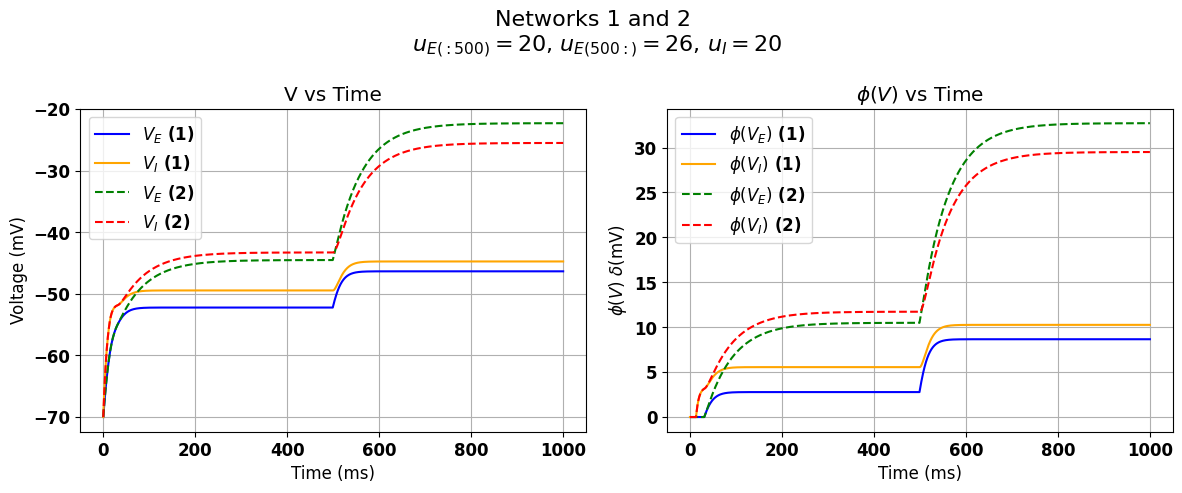
\includegraphics[width=1\textwidth]{images/12-E_input.png}
    \caption{External \textbf{excitatory} input increase after 500ms. $V_I$ unclapmed \\
        \textcolor{red}{Excitatory} potentials are red, \textcolor{blue}{Inhibitory} potentials are blue.\\
        Network 1 is solid, Network 2 is dashed.}
    \label{fig:e-input-unclamped}
\end{figure*}

Stronger excitatory feedback combined with a relatively higher external
stimulation push the neuron towards an endless excitation, so the
inhibitory neuron by extension begins gauging the runaway activity,
thus stabilising the network. This behaviour can once again be
attributed to a different weight of the synaptic Excitatory feedback.

This experiment kept the network in tact, while stimulating the
excitatory neuron and in both cases the system returned to a
stable state. There is a very short delay before the inhibitory
neuron begins catching up, which according to the Equation 1 and
the observations confirms to us that the inhibitory neuron prevents
the runaway excitation of E.

In this next experiment, we will stimulate
the excitatory neuron once again, but this time clamp the inhibitory
neuron for it to remain at the resting potential. The results of this
simulation are show in \ref{fig:e-input-clamped}.

**WRITE THIS UP**

\begin{figure*}
    \centering
    \captionsetup{justification=centering}
    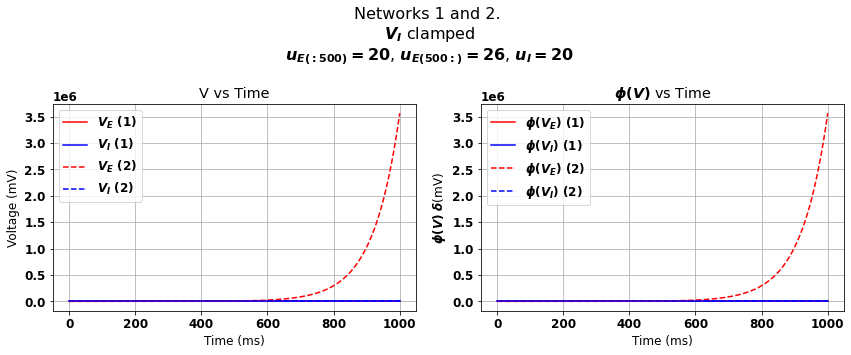
\includegraphics[width=1\textwidth]{images/12-E_input_V_I_clamped.png}
    \caption{External \textbf{excitatory} input increase after 500ms. $V_I$ clapmed \\
        \textcolor{red}{Excitatory} potentials are red, \textcolor{blue}{Inhibitory} potentials are blue.\\
        Network 1 is solid, Network 2 is dashed.}
    \label{fig:e-input-clamped}
\end{figure*}

\subsection{Stabilisation and Paradoxical Inhibition (Q6)}
To sum up findings so far: a network is called ISN if the Excitatory component is unstable
alone, but combined with the inhibitory it is.
The purpose of ISN is to prevent runaway excitation and
maintain the balance in a neural network. Paradoxical inhibition is
a counterintuitive reaction of a network, where external inhibitory input
causes the overall activity of the network to decrease.
Both are most certainly related to the external input, the synaptic weights
and the intrinsic properties of each neuron. 

Based on the simulations, it looks like it is more
affected by the synaptic weights between neurons (including feedback)
 when the system is adapting to the input to reach a stable state. 
In particular, on the excitatory feedback strength relative to the 
inhibitory feedback strength.

Based on the above, it seems reasonable to suppose that 
low $W_{EE}$ to $W_{II}$ ratio ($\le1$)  keeps the network stable and 
high ($>1$) leads to an unstable behaviour, including paradoxical 
inhibition and runaway excitation.

\subsection{Discussion (Q7-8)}
The model has $2\times 6=12$ parameters that can be varied and that 
might influence the behaviour. And while the first 10 of them are 
describing the system, the other 2 - external inputs - can 
vary in time and running simulations on a certain pattern of 
external input does not definitively explain the relationship. 
One alternative way to analyse the model to gain more insight 
into how inhibitory stabilisation relates to the paradoxical inhibition, 
we might look at a more theoretic approach, including 
mathematical analysis of the system. 

\textbf{Assuming the relationship holds, suggest an experiment
to test whether brain networks are in the ISN regime.
Any caveats to the experiment?}

\section{Mathematical Analysis}
In this section, we will provide a mathematical analysis
of the network model and explore the relationship between
the inhibitory stabilisation and paradoxical inhibition.

Assuming, $V > V_0$, we can drop the non-lineraity of the activation
function and expand the expression to do some algebra.

\subsection{Reformulation (Q9)}
To simplify the analysis, we can reformulate the system
of equations describing the network and
express it in the matrix-vector form:

$$
    \frac{d\textbf{V}}{dt}
    = A\textbf{V} + \textbf{x}
    =
    \begin{pmatrix}
        A_{EE} & A_{EI} \\
        A_{IE} & A_{II}
    \end{pmatrix}
    \cdot \begin{pmatrix} \textbf{V}_E \\ \textbf{V}_I \end{pmatrix}
    + \begin{pmatrix} \textbf{x}_E \\ \textbf{x}_I \end{pmatrix}
$$

where $A$ is the matrix of synaptic weights,
and $\textbf{x}$ is the external input.
To find the values of each term, Vs are factored out, and
constant terms are grouped together based on equations (1) and (2).
% grouping terms
$$
    \begin{align*}
        \frac{d\textbf{V}_E}{dt} & = \textbf{V}_E \boxed{\frac{-1 + W_{EE}\beta}{\tau_E}}
        + \textbf{V}_I \boxed{\frac{-W_{EI}\beta}{\tau_E}}                                           \\
                                 & + \boxed{\frac{V_{rest} + V_0\beta(W_{EI}-W_{EE}) + u_E}{\tau_E}}
    \end{align*}
$$

$$
    \begin{align*}
        \frac{d\textbf{V}_I}{dt} & = \textbf{V}_E\boxed{\frac{W_{IE}\beta}{\tau_I}}
        + \textbf{V}_I\boxed{\frac{-1 - W_{II}\beta}{\tau_I}}                                        \\
                                 & + \boxed{\frac{V_{rest} + V_0\beta(W_{II}-W_{IE}) + u_I}{\tau_I}}
    \end{align*}
$$

Now the system can be rewritten in the matrix form:
$$
    \begin{align*}
        \frac{d\textbf{V}}{dt}
        =
        \begin{pmatrix}
            \frac{-1 + w_{EE}\beta}{\tau_E} & \frac{-w_{EI}\beta}{\tau_E}     \\
            \frac{w_{IE}\beta}{\tau_I}      & \frac{-1 - w_{II}\beta}{\tau_I}
        \end{pmatrix}
        \begin{pmatrix}
            \textbf{V}_E \\ \textbf{V}_I
        \end{pmatrix}+
        \\
        +
        \begin{pmatrix}
            \frac{V_{rest} + V_0\beta(W_{EI}-W_{EE}) + u_E}{\tau_E} \\
            \frac{V_{rest} + V_0\beta(W_{II}-W_{IE}) + u_I}{\tau_I}
        \end{pmatrix}
    \end{align*}
$$


\subsection{Steady State (Q10-11)}
The steady state of the system $\textbf{V}^\ast_E,\textbf{V}^\ast_I$ is defined  by
both derivatives being zero. Since $\tau$ are non-zero constant terms, we can drop
them from the equation, and solve for the steady state:

$$
    \begin{pmatrix}
        0 \\ 0
    \end{pmatrix}
    =
    \begin{pmatrix}
        A_{EE} & A_{EI} \\
        A_{IE} & A_{II}
    \end{pmatrix}
    \begin{pmatrix}
        \textbf{V}^\ast_E \\ \textbf{V}^\ast_I
    \end{pmatrix}+
    \begin{pmatrix}
        \textbf{x}_E \\ \textbf{x}_I
    \end{pmatrix}
$$

Rearranging the terms, the solution for steady state voltages:

$$
    \begin{align*}
        \begin{pmatrix}
            \textbf{V}^\ast_E \\ \textbf{V}^\ast_I
        \end{pmatrix}
         & =
        -\begin{pmatrix}
             A_{EE} & A_{EI} \\
             A_{IE} & A_{II}
         \end{pmatrix}^{-1}
        \begin{pmatrix}
            \textbf{x}_E \\ \textbf{x}_I
        \end{pmatrix} \\
         & =
        \frac{-1}{det(A)}
        \begin{pmatrix}
            A_{II}  & -A_{EI} \\
            -A_{IE} & A_{EE}
        \end{pmatrix}
        \begin{pmatrix}
            \textbf{x}_E \\ \textbf{x}_I
        \end{pmatrix}
    \end{align*}
$$

From the solution, we can derive the expression for
inhibitory voltage $V^\ast_I$ in terms of network parameters:

$$
    \begin{align*}
        V^\ast_I
        = \frac{-(- A_{IE}\textbf{x}_E + A_{EE}\textbf{x}_I)}{det(A)}
        = \frac{A_{IE}\textbf{x}_E - A_{EE}\textbf{x}_I}{det(A)}
        % 
        \\
        = \frac{W_{IE}\beta \textbf{x}_E - (W_{EE}\beta - 1) \textbf{x}_I}{det(A)}
    \end{align*}
$$



% A weights
% \begin{pmatrix}
%     -1 + w_{EE}\beta & -w_{EI}\beta     \\
%     w_{IE}\beta      & -1 - w_{II}\beta
% \end{pmatrix}

% X weights
% \begin{pmatrix}
%     V_{rest} + V_0\beta(W_{EI}-W_{EE}) + u_E \\
%     V_{rest} + V_0\beta(W_{II}-W_{IE}) + u_I
% \end{pmatrix}

\section{Conclusion (Q12-13)}

\clearpage
% \newpage
\printbibliography

\clearpage
\appendix
\section{Appendix}
\label{Code}
% \input{images/code.ipynb}

\end{document}
